\section{Key\_\-base$<$ Data, Attribute\-Type $>$ Class Template Reference}
\label{class_key__base}\index{Key_base@{Key\_\-base}}
Functor representing the predicate being not redundant.  


{\tt \#include $<$Key\_\-base.hxx$>$}

Inheritance diagram for Key\_\-base$<$ Data, Attribute\-Type $>$::\begin{figure}[H]
\begin{center}
\leavevmode
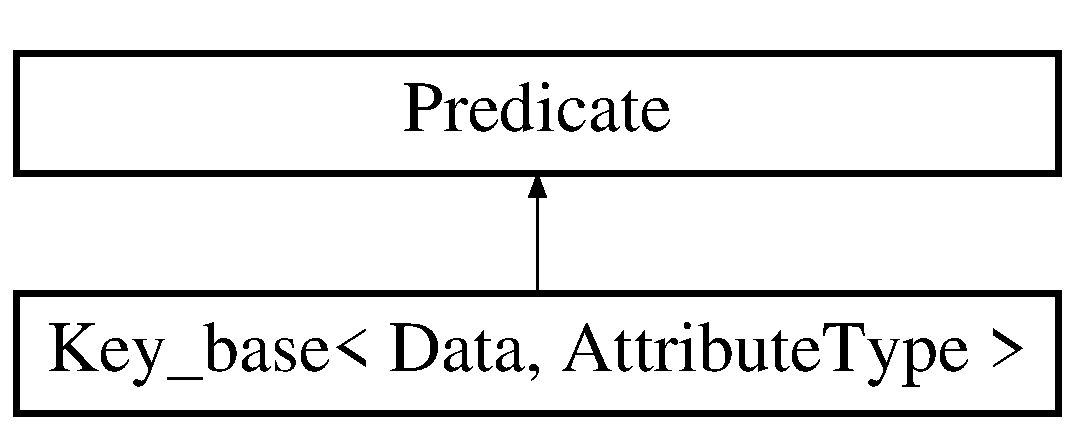
\includegraphics[height=2cm]{class_key__base}
\end{center}
\end{figure}
\subsection*{Public Member Functions}
\begin{CompactItemize}
\item 
template$<$class Input\-DBFormat$>$ {\bf Key\_\-base} (Data \&intable, Input\-DBFormat \&input)\label{class_key__base_f8742868c86280f7f169552d9e2d36fe}

\begin{CompactList}\small\item\em Constructor. \item\end{CompactList}\item 
{\bf $\sim$Key\_\-base} ()\label{class_key__base_8fd75950feb99c6c29008354d893d39c}

\begin{CompactList}\small\item\em Destructor. \item\end{CompactList}\item 
template$<$class Iterator, class Measure$>$ bool {\bf operator()} (Iterator itemset\-It, Measure \&mes\-Cand)
\begin{CompactList}\small\item\em Operator that test if a set of attributes is not redundant. \item\end{CompactList}\end{CompactItemize}
\subsection*{Protected Member Functions}
\begin{CompactItemize}
\item 
template$<$class Iterator$>$ int {\bf count\-Projection} (Iterator it\-Cand)
\begin{CompactList}\small\item\em function used to count the projection of a candidates pointed by the iterator passed in parameter. \item\end{CompactList}\end{CompactItemize}
\subsection*{Protected Attributes}
\begin{CompactItemize}
\item 
int {\bf nb\-Dist\-Tuples}\label{class_key__base_e39c979bb73d9984029b18619e7edeb1}

\begin{CompactList}\small\item\em Number of distinct tuples. \item\end{CompactList}\item 
Data $\ast$ {\bf table}\label{class_key__base_c49571273cb2ae96f540733fdfe05f4d}

\begin{CompactList}\small\item\em the tabular data \item\end{CompactList}\item 
{\bf Recode\-To\-Int}$<$ Attribute\-Type $>$ {\bf num\-Attrib}\label{class_key__base_ed8fae06f994b73f9f9f3eb1ebbac690}

\begin{CompactList}\small\item\em Used to get the numero of the attributes ( 1st, 2nd,...). \item\end{CompactList}\end{CompactItemize}
\subsection*{Classes}
\begin{CompactItemize}
\item 
class {\bf Process\-Tuples}
\begin{CompactList}\small\item\em Functor used to projet all the tuples wrt attributes studied. \item\end{CompactList}\item 
class {\bf project}
\begin{CompactList}\small\item\em Functor used to projet a tuple wrt the set of attributes studied. \item\end{CompactList}\end{CompactItemize}


\subsection{Detailed Description}
\subsubsection*{template$<$class Data, class Attribute\-Type$>$ class Key\_\-base$<$ Data, Attribute\-Type $>$}

Functor representing the predicate being not redundant. 

This functor test if an itemset is a super key. The method used to test if a candidate is a super key is the following one: the functor process the cardinality of the projection wrt the attributes of the candidate. return false if the cardinality is not equal to the number of tuples in the relation.

The template parameter Data is the type of the tablular data. The template parameter Attribute\-Type is the type of the attributes. 



\subsection{Member Function Documentation}
\index{Key_base@{Key\_\-base}!countProjection@{countProjection}}
\index{countProjection@{countProjection}!Key_base@{Key\_\-base}}
\subsubsection{\setlength{\rightskip}{0pt plus 5cm}template$<$class Data, class Attribute\-Type$>$ template$<$class Iterator$>$ int {\bf Key\_\-base}$<$ Data, Attribute\-Type $>$::count\-Projection (Iterator {\em it\-Cand})\hspace{0.3cm}{\tt  [protected]}}\label{class_key__base_2ad0e062e502dd49018ce3f60691f12d}


function used to count the projection of a candidates pointed by the iterator passed in parameter. 

\begin{Desc}
\item[Parameters:]
\begin{description}
\item[{\em it\-Cand}]iterator on the candidate to test. \end{description}
\end{Desc}
\begin{Desc}
\item[Returns:]the cardinality of the projection. \end{Desc}
\index{Key_base@{Key\_\-base}!operator()@{operator()}}
\index{operator()@{operator()}!Key_base@{Key\_\-base}}
\subsubsection{\setlength{\rightskip}{0pt plus 5cm}template$<$class Data, class Attribute\-Type$>$ template$<$class Iterator, class Measure$>$ bool {\bf Key\_\-base}$<$ Data, Attribute\-Type $>$::operator() (Iterator {\em it\-Cand}, Measure \& {\em mes\-Cand})}\label{class_key__base_27f6933ca653e959cea1332231c1ee8a}


Operator that test if a set of attributes is not redundant. 

\begin{Desc}
\item[Parameters:]
\begin{description}
\item[{\em it\-Cand}]iterator (or pointer) on the set of attributes to test wrt the predicate \item[{\em mes\-Cand}]cardinality of the projection on the db of the attributes \end{description}
\end{Desc}


Reimplemented from {\bf Predicate} {\rm (p.\,\pageref{class_predicate_6fb1a75dba2268f75738f335f403e46c})}.

The documentation for this class was generated from the following file:\begin{CompactItemize}
\item 
F:/i\-Zi/problems/key/Key\_\-base.hxx\end{CompactItemize}
